\documentclass{article}

\usepackage{fancyhdr}
\usepackage{extramarks}
\usepackage{amsmath}
\usepackage{amsthm}
\usepackage{amsfonts}
\usepackage{tikz}
\usepackage[plain]{algorithm}
\usepackage{algpseudocode}
\usepackage{listings}
\usepackage{xcolor}
\usepackage[english]{babel}
\usepackage[T1]{fontenc}
\usepackage{lmodern,mathrsfs}
\usepackage{xparse}
\usepackage[inline,shortlabels]{enumitem}
\setlist{topsep=2pt,itemsep=2pt,parsep=0pt,partopsep=0pt}
\usepackage[dvipsnames]{xcolor}
\usepackage[utf8]{inputenc}
\usepackage[a4paper,top=0.5in,bottom=0.2in,left=0.5in,right=0.5in,footskip=0.3in,includefoot]{geometry}
\usepackage[most]{tcolorbox}
\tcbuselibrary{minted} % tcolorbox minted library, required to use the "minted" tcb listing engine (this library is not loaded by the option [most])
\usepackage{minted} % Allows input of raw code, such as Python code
% \usepackage[colorlinks]{hyperref}


\usetikzlibrary{automata,positioning}

\tcbset{
    pythoncodebox/.style={
        enhanced jigsaw,breakable,
        colback=gray!10,colframe=gray!20!black,
        boxrule=1pt,top=2pt,bottom=2pt,left=2pt,right=2pt,
        sharp corners,before skip=10pt,after skip=10pt,
        attach boxed title to top left,
        boxed title style={empty,
            top=0pt,bottom=0pt,left=2pt,right=2pt,
            interior code={\fill[fill=tcbcolframe] (frame.south west)
                --([yshift=-4pt]frame.north west)
                to[out=90,in=180] ([xshift=4pt]frame.north west)
                --([xshift=-8pt]frame.north east)
                to[out=0,in=180] ([xshift=16pt]frame.south east)
                --cycle;
            }
        },
        title={#1}, % Argument of pythoncodebox specifies the title
        fonttitle=\sffamily\bfseries
    },
    pythoncodebox/.default={}, % Default is No title
    %%% Starred version has no frame %%%
    pythoncodebox*/.style={
        enhanced jigsaw,breakable,
        colback=gray!10,coltitle=gray!20!black,colbacktitle=tcbcolback,
        frame hidden,
        top=2pt,bottom=2pt,left=2pt,right=2pt,
        sharp corners,before skip=10pt,after skip=10pt,
        attach boxed title to top text left={yshift=-1mm},
        boxed title style={empty,
            top=0pt,bottom=0pt,left=2pt,right=2pt,
            interior code={\fill[fill=tcbcolback] (interior.south west)
                --([yshift=-4pt]interior.north west)
                to[out=90,in=180] ([xshift=4pt]interior.north west)
                --([xshift=-8pt]interior.north east)
                to[out=0,in=180] ([xshift=16pt]interior.south east)
                --cycle;
            }
        },
        title={#1}, % Argument of pythoncodebox specifies the title
        fonttitle=\sffamily\bfseries
    },
    pythoncodebox*/.default={}, % Default is No title
}

% Custom tcolorbox for Python code (not the code itself, just the box it appears in)
\newtcolorbox{pythonbox}[1][]{pythoncodebox=#1}
\newtcolorbox{pythonbox*}[1][]{pythoncodebox*=#1} % Starred version has no frame

% Custom minted environment for Python code, NOT using tcolorbox
\newminted{python}{autogobble,breaklines,mathescape}

% Custom tcblisting environment for Python code, using the "minted" tcb listing engine
% Adapted from https://tex.stackexchange.com/a/402096
\NewTCBListing{python}{ !O{} !D(){} !G{} }{
    listing engine=minted,
    listing only,
    pythoncodebox={#1}, % First argument specifies the title (if any)
    minted language=python,
    minted options/.expanded={
        autogobble,breaklines,mathescape,
        #2 % Second argument, delimited by (), denotes options for the minted environment
    },
    #3 % Third argument, delimited by {}, denotes options for the tcolorbox
}


%
% Basic Document Settings
%

\topmargin=-0.45in
\evensidemargin=0in
\oddsidemargin=0in
\textwidth=6.5in
\textheight=9.0in
\headsep=0.25in

\linespread{1.1}

\pagestyle{fancy}
\lhead{\hmwkAuthorName}
\chead{\hmwkClass\ (\hmwkClassInstructor): \hmwkTitle}
\rhead{\firstxmark}
\lfoot{\lastxmark}
\cfoot{\thepage}

\renewcommand\headrulewidth{0.4pt}
\renewcommand\footrulewidth{0.4pt}

\setlength\parindent{0pt}

%
% Create Problem Sections
%

\newcommand{\enterProblemHeader}[1]{
	\nobreak\extramarks{}{Problem \arabic{#1} continued on next page\ldots}\nobreak{}
	\nobreak\extramarks{Problem \arabic{#1} (continued)}{Problem \arabic{#1} continued on next page\ldots}\nobreak{}
}

\newcommand{\exitProblemHeader}[1]{
	\nobreak\extramarks{Problem \arabic{#1} (continued)}{Problem \arabic{#1} continued on next page\ldots}\nobreak{}
	\stepcounter{#1}
	\nobreak\extramarks{Problem \arabic{#1}}{}\nobreak{}
}

\setcounter{secnumdepth}{0}
\newcounter{partCounter}
\newcounter{homeworkProblemCounter}
\setcounter{homeworkProblemCounter}{1}
\nobreak\extramarks{Problem \arabic{homeworkProblemCounter}}{}\nobreak{}

%
% Homework Problem Environment
%
% This environment takes an optional argument. When given, it will adjust the
% problem counter. This is useful for when the problems given for your
% assignment aren't sequential. See the last 3 problems of this template for an
% example.
%
\newenvironment{homeworkProblem}[1][-1]{
	\ifnum#1>0
		\setcounter{homeworkProblemCounter}{#1}
	\fi
	\section{Problem \arabic{homeworkProblemCounter}}
	\setcounter{partCounter}{1}
	\enterProblemHeader{homeworkProblemCounter}
}{
	\exitProblemHeader{homeworkProblemCounter}
}

%
% Homework Details
%   - Title
%   - Due date
%   - Class
%   - Section/Time
%   - Instructor
%   - Author
%

\newcommand{\hmwkTitle}{Problem Set\ \#5}
\newcommand{\hmwkDueDate}{Jun 26, 2025}
\newcommand{\hmwkClass}{ECON 219}
\newcommand{\hmwkClassInstructor}{Dr. Sergio Urzua}
\newcommand{\hmwkAuthorName}{\textbf{Alejandro Ouslan}}

%
% Title Page
%

\title{
	\vspace{2in}
	\textmd{\textbf{\hmwkClass:\ \hmwkTitle}}\\
	\normalsize\vspace{0.1in}\small{Due\ on\ \hmwkDueDate}\\
	\vspace{0.1in}\large{\textit{\hmwkClassInstructor}}
	\vspace{3in}
}

\author{\hmwkAuthorName}
\date{}

\renewcommand{\part}[1]{\textbf{\large Part \Alph{partCounter}}\stepcounter{partCounter}\\}

%
% Various Helper Commands
%

% Useful for algorithms
\newcommand{\alg}[1]{\textsc{\bfseries \footnotesize #1}}

% For derivatives
\newcommand{\deriv}[1]{\frac{\mathrm{d}}{\mathrm{d}x} (#1)}

% For partial derivatives
\newcommand{\pderiv}[2]{\frac{\partial}{\partial #1} (#2)}

% Integral dx
\newcommand{\dx}{\mathrm{d}x}

% Alias for the Solution section header
\newcommand{\solution}{\textbf{\large Solution}}

% Probability commands: Expectation, Variance, Covariance, Bias
\newcommand{\E}{\mathrm{E}}
\newcommand{\Var}{\mathrm{Var}}
\newcommand{\Cov}{\mathrm{Cov}}
\newcommand{\Bias}{\mathrm{Bias}}

\begin{document}

\maketitle

\pagebreak

% Problem 1
\begin{homeworkProblem}
	Asume the following smooth production function:
	$$Q= Q(K,L)$$
	with positive marginal productivities. Let $w$ and $r$ the prices of
	labor and capital, respectively.
	\begin{enumerate}
		\item Formulate the problem of minimizing costs subject to the technology.

		      \begin{align*}
			      \min_{K, L} \quad & C = wL + rK       \\
			      \text{s.t.} \quad & Q(K, L) = \bar{Q}
		      \end{align*}
		\item Explain under what conditions you might have to consider the case of corner
		      solution (optimal labor or capital equal to zero). Provide an example.

		      A corner solution arises when either $K = 0$ or $L = 0$. This occurs when:
		      \begin{itemize}
			      \item The marginal productivity of one input is too low relative to its price.
			      \item The isoquants are linear (perfect substitutes) or L-shaped (perfect complements).
		      \end{itemize}

		      \textbf{Example}: For a linear production function:
		      \[
			      Q = aL + bK
		      \]
		      If $\frac{w}{r} > \frac{a}{b}$, then the firm chooses $L = 0$ (uses only capital).
		\item Assuming interior solution present the first order conditions.
		      Provide an economic interpretation to the optimality condition. In you answer,
		      refer to the Lagrange multiplier.

		      \[
			      \mathcal{L} = wL + rK + \lambda (\bar{Q} - Q(K, L))
		      \]

		      \begin{align*}
			      \frac{\partial \mathcal{L}}{\partial L}       & = w - \lambda \frac{\partial Q}{\partial L} = 0 \\
			      \frac{\partial \mathcal{L}}{\partial K}       & = r - \lambda \frac{\partial Q}{\partial K} = 0 \\
			      \frac{\partial \mathcal{L}}{\partial \lambda} & = \bar{Q} - Q(K, L) = 0
		      \end{align*}

		      \[
			      \frac{\frac{\partial Q}{\partial L}}{\frac{\partial Q}{\partial K}} = \frac{w}{r}
			      \quad \Rightarrow \quad MRTS_{L,K} = \frac{w}{r}
		      \]

		      \textbf{Interpretation}:
		      \begin{itemize}
			      \item $\lambda$ is the marginal cost of producing one more unit of output.
			      \item At the optimum, the marginal rate of technical substitution equals the input price ratio.
			      \item The firm equalizes the marginal product per dollar across inputs.
		      \end{itemize}

		\item Provide a graphical representation of the resulting optimal input combination.

		      The optimal bundle lies at the tangency point between the isoquant ($Q = \bar{Q}$) and the isocost line ($wL + rK = C$), where:
		      \[
			      MRTS = \frac{w}{r}
		      \]

		      \begin{center}
			      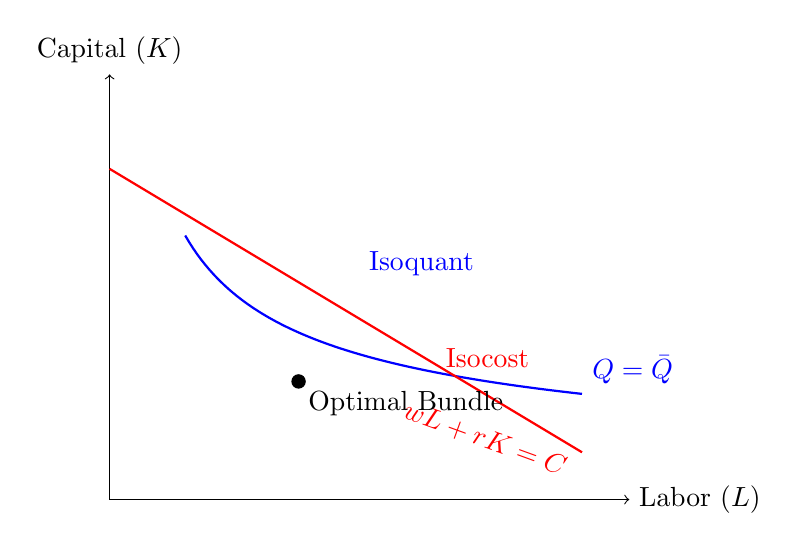
\begin{tikzpicture}[scale=1.2]
				      % Axes
				      \draw[->] (0,0) -- (5.5,0) node[right] {Labor ($L$)};
				      \draw[->] (0,0) -- (0,4.5) node[above] {Capital ($K$)};

				      % Isoquant
				      \draw[thick, blue, domain=0.8:5, samples=100] plot (\x, {2.5/(\x^0.5)}) node[above right] {$Q = \bar{Q}$};

				      % Isocost line
				      \draw[thick, red] (0,3.5) -- (5,0.5) node[below left, rotate=-20] {$wL + rK = C$};

				      % Tangency point
				      \filldraw [black] (2,1.25) circle (2pt) node[below right] {Optimal Bundle};

				      % Labels
				      \node at (3.3,2.5) [blue] {Isoquant};
				      \node at (4,1.5) [red] {Isocost};
			      \end{tikzpicture}
		      \end{center}

		      At this tangency point, the marginal rate of technical substitution equals the input price ratio:
		      \[
			      \frac{MP_L}{MP_K} = \frac{w}{r}
		      \]
		\item Present the second order condition.
		      Use the bordered Hessian:
		      \[
			      H = \begin{bmatrix}
				      0   & Q_L    & Q_K    \\
				      Q_L & Q_{LL} & Q_{LK} \\
				      Q_K & Q_{KL} & Q_{KK}
			      \end{bmatrix}
		      \]
		      The second-order condition requires that $H$ is positive semi-definite at the optimum to ensure a minimum.

		\item Explain how the strict convexity of the isoquants would ensure a minimum cost.
		      Strict convexity of isoquants implies that the cost minimization problem has:
		      \begin{itemize}
			      \item A unique solution.
			      \item No corner solutions.
			      \item A globally cost-minimizing input bundle.
		      \end{itemize}
		\item Explain how quasi-concave production function can generate everywhere strictly convex,
		      downward-sloping isoquants.
		      A strictly quasi-concave production function has convex upper contour sets. This ensures:
		      \begin{itemize}
			      \item Isoquants are strictly convex.
			      \item Isoquants are downward-sloping.
		      \end{itemize}

		\item Now, assume $Q=AL^\alpha K^\beta$. Show that the expansion path (optimal combinations
		      of capital and labor for different isocosts) is characterized by a linear combination.

		      \[
			      \min_{K, L} \quad wL + rK \quad \text{s.t.} \quad Q = AL^\alpha K^\beta = \bar{Q}
		      \]

		      \[
			      \frac{MP_L}{MP_K} = \frac{w}{r} \Rightarrow \frac{\alpha}{\beta} \cdot \frac{K}{L} = \frac{w}{r}
			      \quad \Rightarrow \quad \frac{K}{L} = \frac{\beta}{\alpha} \cdot \frac{w}{r}
		      \]

		      \[
			      K = \left( \frac{\beta}{\alpha} \cdot \frac{w}{r} \right) L
		      \]

		\item Show the previous result holds for all homogeneous production functions.
		      Let $Q(K, L)$ be homogeneous of degree $d > 0$.

		      Because MRTS depends only on $K/L$, solving:
		      \[
			      MRTS = \frac{w}{r}
		      \]
		      yields a constant ratio:
		      \[
			      \frac{K}{L} = \phi(w, r)
			      \quad \Rightarrow \quad K = \phi(w, r) \cdot L
		      \]

		      Therefore, the expansion path is again a \textbf{straight line} through the origin.

	\end{enumerate}
\end{homeworkProblem}
\begin{homeworkProblem}
	Consider the following model:
	$$Y=X\beta + \epsilon$$
	where the standard assumption securing OLS delivers BLUE estimators hold. Assume the error terms
	is normally distributed with mean $0$ and variance $\sigma^2$.
	\begin{enumerate}
		\item Present the likelihood function and optimization problem
		\item Present the first and second order conditions.
		\item Generate a sample of $1000$ observations under the following parameterization:
		      $$Y=X\beta + \epsilon = \beta_0 + \beta_1X + \epsilon$$
		      where $\beta_0= 0.5, \quad \beta_1= -0.75, \quad X \sim (0.5, 2)$, and $\epsilon \sim N(0,1)$.Present
		      summary statistics
		\item Implement the Newton-Raphson algorithm for the MLE problem.
		      \begin{enumerate}
			      \item Report the estimated values for the three parameters.
			      \item Compute the Hessian at the estimated values. How is this connected
			            to the estimators' variance covariance MLE matrix?
		      \end{enumerate}
	\end{enumerate}
\end{homeworkProblem}
\end{document}
